
\appendix
\chapter{Numerical Integration}
\label{sec:num}

We are going to review Numerical Integration indipendently from Optimal Control.

Given an Ordinary Differential Equation (ODE)
\[\dot{x} = f(x,t)\]
with 
\[x(0) = x_0\]
Compute $x(t)\,\,\forall t \in [0, T]$.

If $f$ is \side{Lipshitz continuous} (i.e. the first derivative of the function are bounded) than this problem has an unique solution.

Moreover in $f$ has been omitted the dependency on $u(t)$ given that it is a function of time $t$ and/or $x$.

\section{Numerical Integration Methods}
\subsection{Explicit Euler}
\side{Explicit Euler} is the simplest numerical integration scheme based on the definition of the derivative as:
\[\dot{x} = \lim_{h\to 0} \,\cfrac{x(t+h) - x(t)}{h}\]
with $h$ ``small'' we can approximate $\dot{x}$ with the value on the rhs without the limit and write:
\[h\,\dot{x} \approx x(t+h) - x(t)\]
which means that 
\begin{empheq}[box=%
	\fbox]{gather*}
x(t+h) \approx x(t) + h\,f(x,t)
	\end{empheq}

So the key assumption of the Explicit Euler is to take $h$ sufficiently small in order for it to work but the methods does not specify exactly how small it must be the step. However taking $h$ small means that it will be computationally expensive.

Moreover it is not very accurate (first order method).

\subsection{Mid-Point Method}
The \side{Mid-Point Method} is slightly better than the Explicit Euler. 

You take a first step to reach the middle of the time step, you look at the value of $\dot{x}$ in the middle and this is the value that you use in the whole time step.

So you go back and you integrate the time step using the value of $\dot{x}$ that you computed in the middle of the step:
\begin{empheq}[box=%
	\fbox]{align*}
k_1 &= f(x_0, t_0)\\
k_2 &= f\left(x_0 + \cfrac{h}{2}\,k_1, t_0 + \cfrac{h}{2}\right)\\
x_1 &= x_0 + h\,k_2
\end{empheq}
\begin{figure}[!h]
\centering
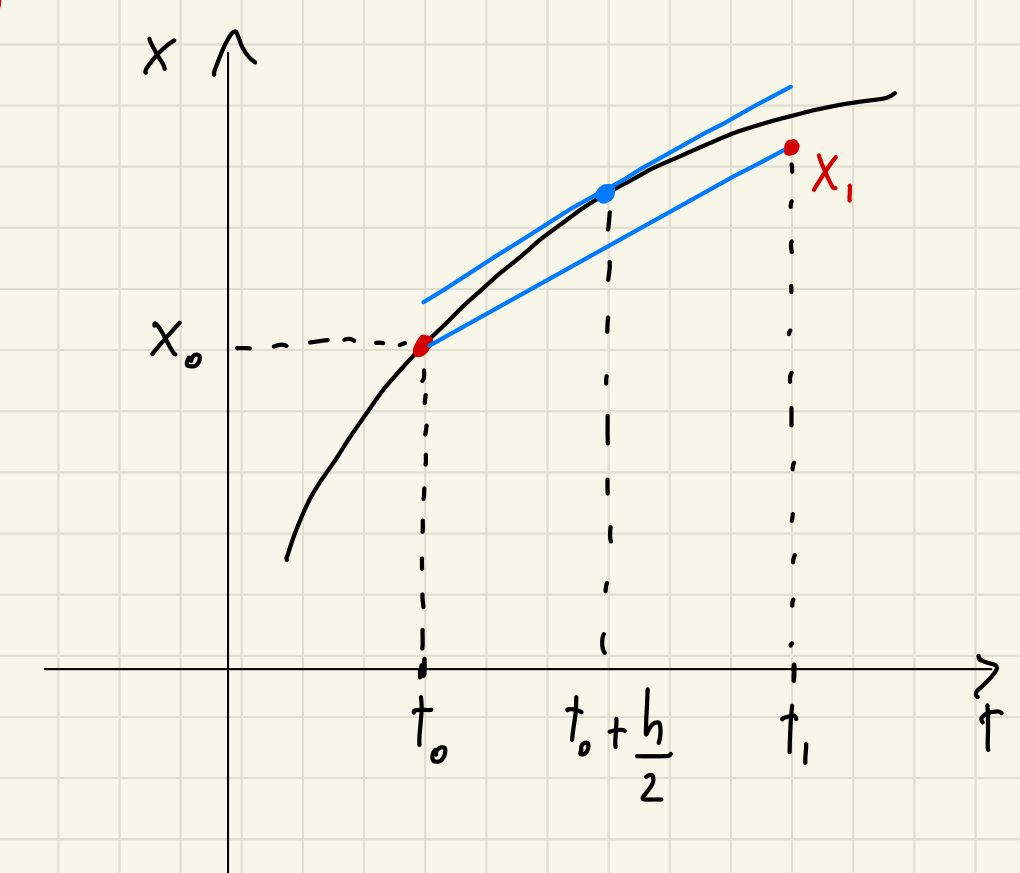
\includegraphics[width=.4\textwidth]{image0A04}
\caption{Mid-Point method: find the midpoint of the interval, compute derivative, compute area starting from the initial point of the interval using the slope of the midpoint}
\end{figure}
\begin{enumerate}
\item Use the slope in the middle of the step to integrate forward
\item Estimate $x\left(t_0 + \cfrac{h}{2}\right)$ with the slop at $t_0$
\item Second order method (order 2)
\item Need 2 function evaluation for each step
\end{enumerate}

The theory that allows us to state that almost always the midpoint method is better than explicit Euler is the theory of numerical integration scheme.

\subsection{Runge-Kutta Methods}
The Euler method and midpoint method are both specific cases of \side{Runge-Kutta method}.

The RK methods are based on the following equations:
\begin{empheq}[box=%
\fbox]{align*}
x_{n+1} &= x_n + h\,\sum_{i=1}^q \,b_i\,k_i\\
k_i &= f\left(x_n\,+\,h\sum_{j=1}^q\,a_{ij}\,k_j , t_n + c_i\,h\right)
\end{empheq}
where:
\begin{itemize}
\item $q\,\,$ is the order of the method (not to be confused with the consistency order of the method)
\item For $q = 1$ we recover Euler by setting ($b_1 = 1, a_{11} = 0, c_1 = 0$)
\item The Mid-point method is an RK method of order $q = 2$
\item If $a_{ij} = 0\,\, \forall j\ge i$ the method is called \side{explicit method}.

Otherwise the method is called \side{implicit method} (need to solve system of equations because to compute $k_i$ you need to know the value of other $k$ that are all interdependent).
\item For $q > 1$ there exist many versions of the same order.
\item the term $\sum_{i=1}^q\,b_i\,k_i$ is an approximation of $\dot{x}$ with an weighted average of $k_i$, with weights $b_i$.

Where 
\[\sum b_i = 1 \qquad b_i \ge 0\]
\end{itemize}

Therefore to define a RK method you need all the values of parameter $a, b$ and $c$. Tipically these parameters are stored in a so called \side{Butcher Tableau}.

\[
\begin{NiceArray}{c|ccc}
c_1& a_{11}&\Cdots & a_{1q}\\
\Vdots &  \Vdots& \Ddots& \Vdots\\
c_q& a_{q1} & \Cdots & a_{qq}\\
\midrule
& b_1 &\Cdots&b_q
\end{NiceArray}
\]
\begin{itemize}
\item Once you have this tableau you have uniquely defined the RK method
\item Most common explicit RK4 method and takes the form
\begin{empheq}[box=%
\fbox]{align*}
k_1 &= f(x_n,\,t_n)\\
k_2 &= f\left(x_n + \cfrac{1}{2} h\,k_1, t_n + \cfrac{1}{2}\,h\right)\\
k_3 &= f\left(x_n + \cfrac{1}{2} h\,k_2, t_n + \cfrac{1}{2} h\right)\\
k_4 &= f(x_n + h\,k_3, t_n\,+\,h)\\
x_{n+1} &= x_n + \cfrac{h}{6} (k_1 + 2\,k_2 + 2\,k_3+k_4)
\end{empheq}
and it can be uniquely defined by the Butcher Tableau:
\[
\begin{NiceArray}{c|cccc}
0& \\
\sfrac{1}{2}& \sfrac{1}{2} & \\
\sfrac{1}{2}& 0 & \sfrac{1}{2}\\
1 & 0 & 0 & 1\\
\midrule
& \sfrac{1}{6} &\sfrac{1}{3}&\sfrac{1}{3}&\sfrac{1}{6}
\end{NiceArray}
\]
The main reason this method is so common comes from the fact that it draws the limit for which you get a method that has the same consistency order of the order of the RK scheme (i.e. for $p\ge5 \,\nexists \text{method with } q=p$).
\end{itemize}

\begin{minipage}{0.475\textwidth}
\centering
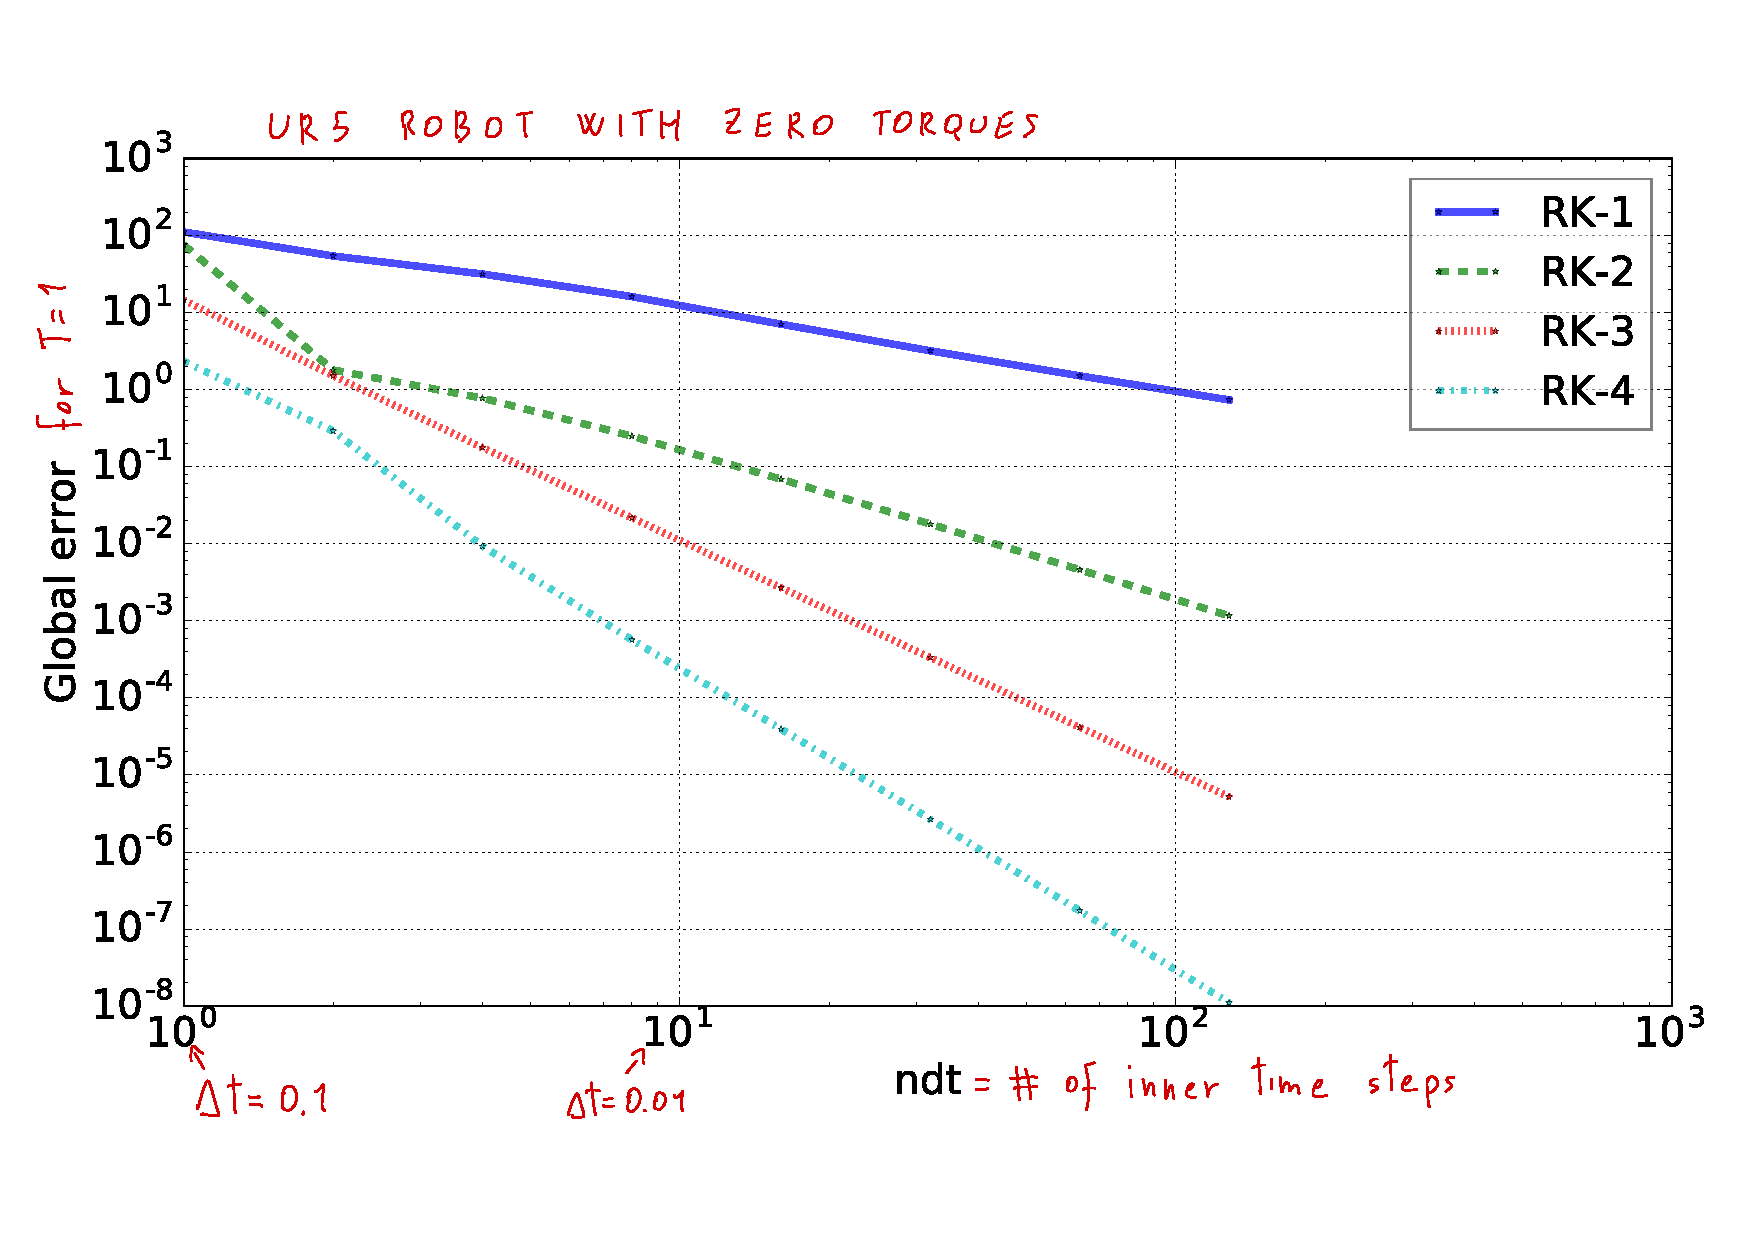
\includegraphics[width=\textwidth]{image0A01.pdf}
\end{minipage}
\hfill
\begin{minipage}{0.475\textwidth}
\centering
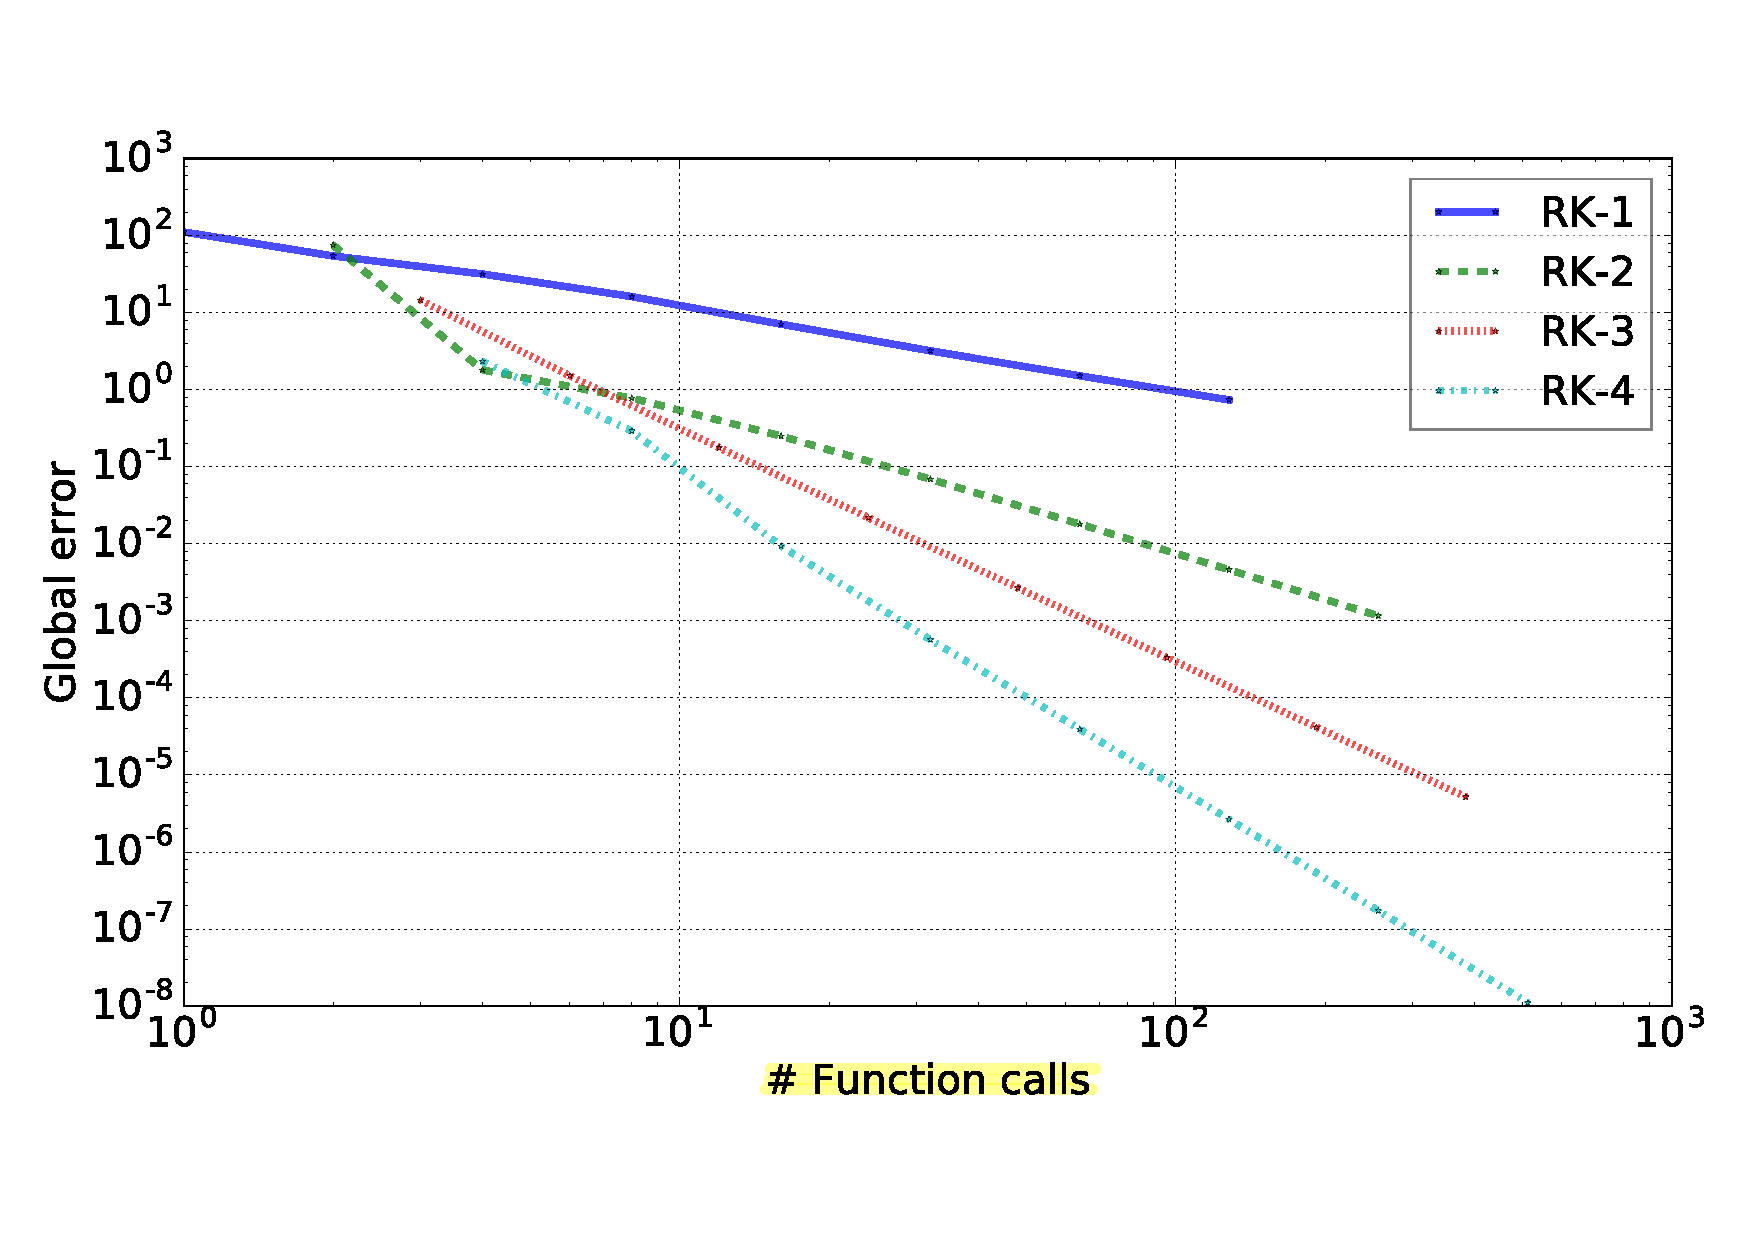
\includegraphics[width=\textwidth]{image0A02.pdf}
\end{minipage}


\section{Properties of Integration Schemes}
Definitions:
\begin{itemize}
\item{\makebox[5cm]{Integrator output:\hfill} $\hat{x}(t, t_0, x(t_0))$}
\item{\makebox[5cm]{Exact trajectory:\hfill} $x(t)$}
\item{\makebox[5cm]{Local integration error:\hfill} $e(t) = x(t) - \hat{x}(t, t-h, x(t-h))$}
\item{\makebox[5cm]{Global integration error:\hfill} $E(t) = x(t) - \hat{x}(t, t_0, x(t_0))$ }
\end{itemize}
Now that we have defined these two error we can talk about the properties of integration schemes which are:
\begin{enumerate}
\item \side{Convergence}.

Convergence is the basic properties that ensures that as the time step that you use for integration goes to zero the global error should go to zero as well:
\[\lim_{h\to0} \,E = 0\]
It is not a very difficult property to achieve. Basically all the integration methods have this property.
\item \side{Consistency order} p.

Tells you how quickly the error goes to zero. In particular it is formulated using the local error.
In particular the limit of the local error should go to zero as a polynomial of the time step:
\[\lim_{h\to0}\,e=O(h^{p+1})\qquad p>0\]
So when we refer to a method order 1 or 2 we refer to the value of p on the above definition.
\item \side{Stability}.

There is no clear definition of stability.  But we can approximately define it as the global error remains bounded as we keep integrate ($t\to\infty$)
\end{enumerate}

From this definitions we can now quantify the performance of each method through the notion of consistency order.
\begin{itemize}
\item The local error for Explicit Euler takes the form:
\[e(t) \triangleq x(t+h) - \hat{x}(t+h, t, x(t)) = x_{n+1} - \hat{x}_{n+1}(x_n) = e_{n+1}\]
where 
\[x_n \triangleq x(t_n)\]
So we can reformulate the expression as:
\[\hat{x}_{n+1} = x_n + h\,f(x_n, t_n)\]
Let us express $x_n$ with a Taylor series around $x_n$:
\[x_{n+1} = x_n + h\,\dot{x}_n + O(h^2)\]
Whatever remains is something in the order of $h^2$.
And Finally we can compute the error with the expression above:
\begin{align*}
e_{n+1} &= x_{n+1} - \hat{x}_{n+1}\\
&= \cancel{x_n} + \cancel{h\,\dot{x}_n} + O(h^2) - \cancel{x_n} - \cancel{h\,f(x_n,t_n)}\\
&= O(h^2)
\end{align*}
So this means that the method is of order 1 (i.e. $p = 1$)

\item The local error for Mid-point method takes the form:
\[e(t) = x(t+h) - \hat{x}(t+h, t, x(t)) = x_{n+1} - \hat{x}_{n+1}(x_n)\]
where
\begin{align*}
k_1 &\triangleq f(x_n, t_n) = \dot{x}_n\\
\hat{x}_{n+1} &= x_n\,+h\,f\left(x_n+\cfrac{h}{2}\,k_1, t_n + \cfrac{h}{2}\right)\\
f &= \dot{x}\\
\dot{f} &= \left(\pd{f_n}{x_n}\,\td{x_n}{t_n} + \pd{f_n}{t_n}\right) = \ddot{x}
\end{align*}
Let us express $x_{n+1}$ with the Taylor series around $x_n$:
\[x_{n+1} = x_n + h\,\dot{x}_n + \cfrac{h^2}{2}\,\ddot{x}_n + O(h^3)\]
And let us express $f(x_n+\cfrac{h}{2}\,\dot{x}_n, t_n + \cfrac{h}{2})$ with the Taylor series around $(x_n, t_n)$:
\begin{align*}
f\left(x_n+\cfrac{h}{2}\,\dot{x}_n, t_n + \cfrac{h}{2}\right) &=f(x_n, t_n) + \pd{f_n}{x_n}\,\cfrac{h}{2}\,\dot{x}_n \, +\, \pd{f_n}{t_n}\,\cfrac{h}{2} + O(h^2)\\
&= \dot{x}_n + \cfrac{h}{2}\,\ddot{x}_n + O(h^2)
\end{align*}
We can finally write the error using the expressions above:
\begin{align*}
e_{n+1} &= x_{n+1} - \hat{x}_{n+1} \\
&= \cancel{x_n} + \cancel{h\,\dot{x}_n} + \cfrac{h^2}{2}\,\ddot{x}_n\,+O(h^3) - \left(\cancel{x_n}\,+ h\,\left(\cancel{\dot{x}_n}\,+\cfrac{h}{2}\,\ddot{x}_n + O(h^2) \right)\right)\\
&= O(h^3)
\end{align*}
So this means that the method is of order 2 (i.e. $p = 2$)
\end{itemize}